\begin{scanpage}{0133}{116}
\noindent\begin{minipage}[t]{.48\linewidth}\vspace{0pt}\centering
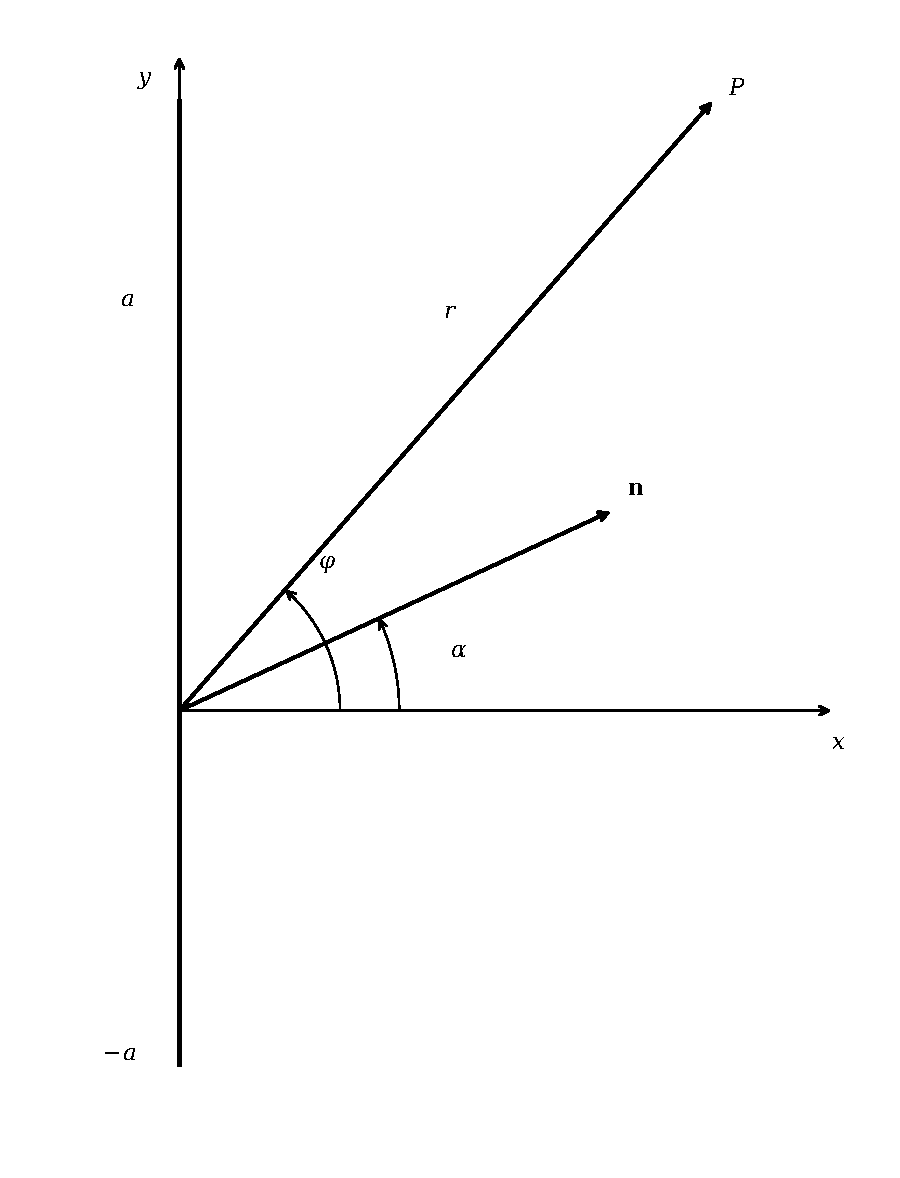
\includegraphics[width=.58\linewidth]{images/recreated/b-0133-fig45.pdf}

\raggedright Figure 45. The transverse cross section of a strip with the plane $xoy$, $x=0$, $y=a$ and $x=0$, $y=-a$ are the coordinates of the strip's edge; $\mathbf n$ is the normal to the incident plane wave front.
\end{minipage}\hfill\begin{minipage}[t]{.48\linewidth}\vspace{0pt}
In \S\ 6 approximation expressions were found for the fringing field in the far zone which did not consider the interaction of the edges. In the case of E-polarization of the incident wave $(\mathbf E_0\parallel Oz)$, these expressions may be represented in the form
\end{minipage}
\[\left.\begin{aligned}E_z=-H_\varphi&=E_{0z}[f(1)e^{ika(\sin\alpha-\sin\varphi)}\\&\quad+f(2)e^{-ika(\sin\alpha-\sin\varphi)}]\frac{e^{i(kr+\pi/4)}}{\sqrt{2\pi kr}},\\E_\varphi=H_z&=0,\end{aligned}\right\}\tag{20.02}\]
and in the case of H-polarization $(\mathbf H_0\parallel Oz)$
\[\left.\begin{aligned}H_z=E_\varphi&=H_{0z}[g(1)e^{ika(\sin\alpha-\sin\varphi)}\\&\quad+g(2)e^{-ika(\sin\alpha-\sin\varphi)}]\frac{e^{i(kr+\pi/4)}}{\sqrt{2\pi kr}},\\H_\varphi=E_z&=0.\end{aligned}\right\}\tag{20.03}\]
Let us recall that the functions $f$ and $g$ included here are determined in the region $|\varphi|<\frac\pi2$ (when $|\alpha|<\frac\pi2$) by the following relationships:
\[f(1)=\frac{\cos\frac{\alpha+\varphi}2-\sin\frac{\alpha-\varphi}2}{\sin\alpha-\sin\varphi},\quad f(2)=-\frac{\cos\frac{\alpha+\varphi}2+\sin\frac{\alpha-\varphi}2}{\sin\alpha-\sin\varphi},\tag{20.04}\]
\[g(1)=-f(2),\quad g(2)=-f(1).\tag{20.05}\]
The first terms in Equations (20.02) and (20.03) describe cylindrical waves diverging from edge 1 $(y=a)$, and the second terms describe the cylindrical waves diverging from edge 2 $(y=-a)$. The
\end{scanpage}
